\documentclass[twoside]{book}

% Packages required by doxygen
\usepackage{calc}
\usepackage{doxygen}
\usepackage{graphicx}
\usepackage[utf8]{inputenc}
\usepackage{makeidx}
\usepackage{multicol}
\usepackage{multirow}
\usepackage{textcomp}
\usepackage[table]{xcolor}

% Font selection
\usepackage[T1]{fontenc}
\usepackage{mathptmx}
\usepackage[scaled=.90]{helvet}
\usepackage{courier}
\usepackage{amssymb}
\usepackage{sectsty}
\renewcommand{\familydefault}{\sfdefault}
\allsectionsfont{%
  \fontseries{bc}\selectfont%
  \color{darkgray}%
}
\renewcommand{\DoxyLabelFont}{%
  \fontseries{bc}\selectfont%
  \color{darkgray}%
}

% Page & text layout
\usepackage{geometry}
\geometry{%
  a4paper,%
  top=2.5cm,%
  bottom=2.5cm,%
  left=2.5cm,%
  right=2.5cm%
}
\tolerance=750
\hfuzz=15pt
\hbadness=750
\setlength{\emergencystretch}{15pt}
\setlength{\parindent}{0cm}
\setlength{\parskip}{0.2cm}
\makeatletter
\renewcommand{\paragraph}{%
  \@startsection{paragraph}{4}{0ex}{-1.0ex}{1.0ex}{%
    \normalfont\normalsize\bfseries\SS@parafont%
  }%
}
\renewcommand{\subparagraph}{%
  \@startsection{subparagraph}{5}{0ex}{-1.0ex}{1.0ex}{%
    \normalfont\normalsize\bfseries\SS@subparafont%
  }%
}
\makeatother

% Headers & footers
\usepackage{fancyhdr}
\pagestyle{fancyplain}
\fancyhead[LE]{\fancyplain{}{\bfseries\thepage}}
\fancyhead[CE]{\fancyplain{}{}}
\fancyhead[RE]{\fancyplain{}{\bfseries\leftmark}}
\fancyhead[LO]{\fancyplain{}{\bfseries\rightmark}}
\fancyhead[CO]{\fancyplain{}{}}
\fancyhead[RO]{\fancyplain{}{\bfseries\thepage}}
\fancyfoot[LE]{\fancyplain{}{}}
\fancyfoot[CE]{\fancyplain{}{}}
\fancyfoot[RE]{\fancyplain{}{\bfseries\scriptsize Generated on Thu Aug 22 2013 17\-:27\-:48 for Hash\-Table by Doxygen }}
\fancyfoot[LO]{\fancyplain{}{\bfseries\scriptsize Generated on Thu Aug 22 2013 17\-:27\-:48 for Hash\-Table by Doxygen }}
\fancyfoot[CO]{\fancyplain{}{}}
\fancyfoot[RO]{\fancyplain{}{}}
\renewcommand{\footrulewidth}{0.4pt}
\renewcommand{\chaptermark}[1]{%
  \markboth{#1}{}%
}
\renewcommand{\sectionmark}[1]{%
  \markright{\thesection\ #1}%
}

% Indices & bibliography
\usepackage{natbib}
\usepackage[titles]{tocloft}
\setcounter{tocdepth}{3}
\setcounter{secnumdepth}{5}
\makeindex

% Hyperlinks (required, but should be loaded last)
\usepackage{ifpdf}
\ifpdf
  \usepackage[pdftex,pagebackref=true]{hyperref}
\else
  \usepackage[ps2pdf,pagebackref=true]{hyperref}
\fi
\hypersetup{%
  colorlinks=true,%
  linkcolor=blue,%
  citecolor=blue,%
  unicode%
}

% Custom commands
\newcommand{\clearemptydoublepage}{%
  \newpage{\pagestyle{empty}\cleardoublepage}%
}


%===== C O N T E N T S =====

\begin{document}

% Titlepage & ToC
\hypersetup{pageanchor=false}
\pagenumbering{roman}
\begin{titlepage}
\vspace*{7cm}
\begin{center}%
{\Large Hash\-Table \\[1ex]\large H\-W 10 }\\
\vspace*{1cm}
{\large Generated by Doxygen 1.8.4}\\
\vspace*{0.5cm}
{\small Thu Aug 22 2013 17:27:48}\\
\end{center}
\end{titlepage}
\clearemptydoublepage
\tableofcontents
\clearemptydoublepage
\pagenumbering{arabic}
\hypersetup{pageanchor=true}

%--- Begin generated contents ---
\chapter{H\-W11\-: Implementing a spell checker}
\label{index}\hypertarget{index}{}\begin{DoxyAuthor}{Author}
Kevin Mc\-Swiggen and Mars Park
\end{DoxyAuthor}
\hypertarget{index_intro_sec}{}\section{Introduction}\label{index_intro_sec}
If given a list of all words, it is possible to insert all those words in a hash table. Then, we can check if an abitrary word is a legitimate word by testing if it exists in the hash table.

The spell checker takes a step further and not only checks if the word exists in the hash but also suggests correct words. This spell checker does this by checking if there is a wrong letter in the word. When a word is not found in the dictionary, the spell checker will look up all variants that can be generated by changing one character. If the spell checker finds a match in the dictionary with one of these variants, it adds to the output line.

Our spell checker can be run using any of four choices of set implementation that inherit from the \hyperlink{class_abstract_set}{Abstract\-Set} abstract template class. \hyperlink{class_std_hash_set}{Std\-Hash\-Set} and \hyperlink{class_std_tree_set}{Std\-Tree\-Set} are wrapper classes for the S\-T\-L classes unordered\-\_\-set$<$\-T$>$ and set$<$\-T$>$ respectively. The \hyperlink{class_hash_set}{Hash\-Set} class is a custom implementation of a linear-\/probing hash set. When the key for a given element is taken, the insertion point advances until finding an unocupied index of the hash table. After the hash set becomes sufficiently full, it will resize the hash table and rehash the elements in the hash set to keep long clusters of keys from negatively impacting the performance of the hash set. The \hyperlink{class_tree_set}{Tree\-Set} class is a custom implementation of an A\-V\-L self-\/balancing binary search tree. When the subtrees of any node differ in height by more than 1, the tree is re-\/balanced by rotating through the node appropriately.\hypertarget{index_use_sec}{}\section{Usage}\label{index_use_sec}
The spell checking can be run using\-: \begin{DoxyVerb}./myspell [-d] [-h / -t/ -T / -H] dictionary
\end{DoxyVerb}


where
\begin{DoxyItemize}
\item -\/d prints information about the data structure used to represent the dictionary. \char`\"{}dictionary\char`\"{} is the file name of the dictionary.
\item -\/h Prints out\-: \char`\"{}n expansions, load factor f, c collisions, longest run l\char`\"{} where n, c, and l are integers, and f is a floating-\/point (double) number, printed in the default format.
\item -\/t Prints out a single line containing useful information about the structure of the tree, including its height.
\item -\/\-T Prints \char`\"{}\-No statistics available\char`\"{}
\item -\/\-H Prints \char`\"{}\-No statistics available\char`\"{}
\end{DoxyItemize}\hypertarget{index_change_sec}{}\section{Changes made to myspell program}\label{index_change_sec}
Myspell now keeps track of errors which have been previously seen and only prints out spelling corrections for novel errors.

Myspell is now implemented using \hyperlink{class_abstract_set}{Abstract\-Set}, and takes flages (-\/h, -\/\-H, -\/t, -\/\-T) to specify which type of set should be used to store the dictionary and set of previously-\/seen errors. The dictionary and error sets are constructed on the heap as the requested type.

Debugging information printed out by the -\/d flag now depends on which type of set is used to store the words.

performance\-\_\-page Peformance comparisons between the different sets can be found on their own page. 
\chapter{Performance comparisons between different sets}
\label{performance}
\hypertarget{performance}{}
\begin{DoxyAuthor}{Author}
Kevin Mc\-Swiggen and Mars Park
\end{DoxyAuthor}
The performance tests were run from the C\-S lab computer, oak.\-cs.\-hmc.\-edu, and was compiled on knuth. We used three different files to do a performance comparison. The three different files were decided based on the length of the text. The first text file is The Republic by Plato which is 25,000 lines, the second text file is The Bible which is 100,000 lines, and the third text is the works of William Shakespeare which is 125,000 lines. The dictionary we used for spelling checking is an alphabetically ordered list of 35,000 words. The times were taken from code compiled with -\/\-O3.

The times for running myspell with a specific set are at the bottom and will be referred to.

For all three files, we notice that using \hyperlink{class_hash_set}{Hash\-Set} or \hyperlink{class_std_hash_set}{Std\-Hash\-Set} are quicker than using \hyperlink{class_tree_set}{Tree\-Set} or \hyperlink{class_std_tree_set}{Std\-Tree\-Set}. We believe that is true because hash tables take constant time to look up while trees take an expected time of log(\-N) to look up where N is the number of elements in the tree. It is difficult to make a conclusion between \hyperlink{class_hash_set}{Hash\-Set} and \hyperlink{class_std_hash_set}{Std\-Hash\-Set} or between \hyperlink{class_tree_set}{Tree\-Set} and \hyperlink{class_std_tree_set}{Std\-Tree\-Set} because the times are close enough that there are overlaps between the two within many runs. We consider that as a success.



 \subsection*{Plato's \char`\"{}\-The Republic\char`\"{} }

./myspell -\/d -\/h ispell.\-words $<$ test\-Files/republic.\-txt 0.\-33s user 0.\-02s system 92\% cpu 0.\-377 total ./myspell -\/d -\/h ispell.\-words $<$ test\-Files/republic.\-txt 0.\-31s user 0.\-02s system 92\% cpu 0.\-358 total ./myspell -\/d -\/h ispell.\-words $<$ test\-Files/republic.\-txt 0.\-29s user 0.\-02s system 92\% cpu 0.\-337 total ./myspell -\/d -\/h ispell.\-words $<$ test\-Files/republic.\-txt 0.\-32s user 0.\-02s system 93\% cpu 0.\-375 total ./myspell -\/d -\/h ispell.\-words $<$ test\-Files/republic.\-txt 0.\-34s user 0.\-03s system 93\% cpu 0.\-397 total

./myspell -\/d -\/t ispell.\-words $<$ test\-Files/republic.\-txt 1.\-02s user 0.\-02s system 97\% cpu 1.\-070 total ./myspell -\/d -\/t ispell.\-words $<$ test\-Files/republic.\-txt 0.\-87s user 0.\-08s system 96\% cpu 0.\-986 total ./myspell -\/d -\/t ispell.\-words $<$ test\-Files/republic.\-txt 0.\-95s user 0.\-02s system 97\% cpu 0.\-994 total ./myspell -\/d -\/t ispell.\-words $<$ test\-Files/republic.\-txt 0.\-90s user 0.\-02s system 97\% cpu 0.\-950 total ./myspell -\/d -\/t ispell.\-words $<$ test\-Files/republic.\-txt 0.\-95s user 0.\-02s system 97\% cpu 1.\-000 total

./myspell -\/d -\/\-H ispell.\-words $<$ test\-Files/republic.\-txt 0.\-34s user 0.\-03s system 93\% cpu 0.\-391 total ./myspell -\/d -\/\-H ispell.\-words $<$ test\-Files/republic.\-txt 0.\-36s user 0.\-02s system 94\% cpu 0.\-405 total ./myspell -\/d -\/\-H ispell.\-words $<$ test\-Files/republic.\-txt 0.\-33s user 0.\-02s system 93\% cpu 0.\-375 total ./myspell -\/d -\/\-H ispell.\-words $<$ test\-Files/republic.\-txt 0.\-35s user 0.\-06s system 92\% cpu 0.\-442 total ./myspell -\/d -\/\-H ispell.\-words $<$ test\-Files/republic.\-txt 0.\-31s user 0.\-03s system 93\% cpu 0.\-364 total

./myspell -\/d -\/\-T ispell.\-words $<$ test\-Files/republic.\-txt 0.\-86s user 0.\-02s system 97\% cpu 0.\-899 total ./myspell -\/d -\/\-T ispell.\-words $<$ test\-Files/republic.\-txt 0.\-80s user 0.\-03s system 96\% cpu 0.\-858 total ./myspell -\/d -\/\-T ispell.\-words $<$ test\-Files/republic.\-txt 0.\-70s user 0.\-03s system 96\% cpu 0.\-748 total ./myspell -\/d -\/\-T ispell.\-words $<$ test\-Files/republic.\-txt 0.\-79s user 0.\-02s system 96\% cpu 0.\-847 total ./myspell -\/d -\/\-T ispell.\-words $<$ test\-Files/republic.\-txt 0.\-72s user 0.\-02s system 96\% cpu 0.\-764 total 

 \subsection*{The King James Bible }

./myspell -\/d -\/h ispell.\-words $<$ test\-Files/kjb.\-txt 0.\-83s user 0.\-05s system 95\% cpu 0.\-922 total ./myspell -\/d -\/h ispell.\-words $<$ test\-Files/kjb.\-txt 0.\-75s user 0.\-04s system 94\% cpu 0.\-835 total ./myspell -\/d -\/h ispell.\-words $<$ test\-Files/kjb.\-txt 0.\-80s user 0.\-04s system 94\% cpu 0.\-885 total ./myspell -\/d -\/h ispell.\-words $<$ test\-Files/kjb.\-txt 0.\-80s user 0.\-05s system 94\% cpu 0.\-898 total ./myspell -\/d -\/h ispell.\-words $<$ test\-Files/kjb.\-txt 0.\-84s user 0.\-06s system 93\% cpu 0.\-960 total

./myspell -\/d -\/t ispell.\-words $<$ test\-Files/kjb.\-txt 1.\-80s user 0.\-03s system 97\% cpu 1.\-873 total ./myspell -\/d -\/t ispell.\-words $<$ test\-Files/kjb.\-txt 1.\-97s user 0.\-04s system 97\% cpu 2.\-053 total ./myspell -\/d -\/t ispell.\-words $<$ test\-Files/kjb.\-txt 2.\-18s user 0.\-03s system 97\% cpu 2.\-263 total ./myspell -\/d -\/t ispell.\-words $<$ test\-Files/kjb.\-txt 1.\-78s user 0.\-04s system 97\% cpu 1.\-865 total ./myspell -\/d -\/t ispell.\-words $<$ test\-Files/kjb.\-txt 1.\-86s user 0.\-04s system 97\% cpu 1.\-940 total

./myspell -\/d -\/\-H ispell.\-words $<$ test\-Files/kjb.\-txt 0.\-88s user 0.\-04s system 94\% cpu 0.\-970 total ./myspell -\/d -\/\-H ispell.\-words $<$ test\-Files/kjb.\-txt 0.\-85s user 0.\-04s system 94\% cpu 0.\-948 total ./myspell -\/d -\/\-H ispell.\-words $<$ test\-Files/kjb.\-txt 0.\-77s user 0.\-03s system 94\% cpu 0.\-848 total ./myspell -\/d -\/\-H ispell.\-words $<$ test\-Files/kjb.\-txt 0.\-87s user 0.\-04s system 95\% cpu 0.\-947 total ./myspell -\/d -\/\-H ispell.\-words $<$ test\-Files/kjb.\-txt 0.\-83s user 0.\-04s system 95\% cpu 0.\-917 total

./myspell -\/d -\/\-T ispell.\-words $<$ test\-Files/kjb.\-txt 1.\-50s user 0.\-05s system 97\% cpu 1.\-602 total ./myspell -\/d -\/\-T ispell.\-words $<$ test\-Files/kjb.\-txt 1.\-74s user 0.\-03s system 97\% cpu 1.\-818 total ./myspell -\/d -\/\-T ispell.\-words $<$ test\-Files/kjb.\-txt 1.\-67s user 0.\-04s system 97\% cpu 1.\-758 total ./myspell -\/d -\/\-T ispell.\-words $<$ test\-Files/kjb.\-txt 1.\-93s user 0.\-03s system 97\% cpu 2.\-006 total ./myspell -\/d -\/\-T ispell.\-words $<$ test\-Files/kjb.\-txt 1.\-66s user 0.\-04s system 97\% cpu 1.\-753 total 

 \subsection*{The works of William Shakespeare }

./myspell -\/d -\/h ispell.\-words $<$ test\-Files/shakespeare.\-txt 1.\-26s user 0.\-12s system 92\% cpu 1.\-495 total ./myspell -\/d -\/h ispell.\-words $<$ test\-Files/shakespeare.\-txt 1.\-07s user 0.\-09s system 90\% cpu 1.\-281 total ./myspell -\/d -\/h ispell.\-words $<$ test\-Files/shakespeare.\-txt 1.\-30s user 0.\-09s system 91\% cpu 1.\-504 total ./myspell -\/d -\/h ispell.\-words $<$ test\-Files/shakespeare.\-txt 1.\-16s user 0.\-09s system 92\% cpu 1.\-364 total ./myspell -\/d -\/h ispell.\-words $<$ test\-Files/shakespeare.\-txt 1.\-36s user 0.\-09s system 92\% cpu 1.\-567 total

./myspell -\/d -\/t ispell.\-words $<$ test\-Files/shakespeare.\-txt 3.\-92s user 0.\-08s system 97\% cpu 4.\-113 total ./myspell -\/d -\/t ispell.\-words $<$ test\-Files/shakespeare.\-txt 4.\-69s user 0.\-09s system 97\% cpu 4.\-893 total ./myspell -\/d -\/t ispell.\-words $<$ test\-Files/shakespeare.\-txt 3.\-45s user 0.\-07s system 96\% cpu 3.\-628 total ./myspell -\/d -\/t ispell.\-words $<$ test\-Files/shakespeare.\-txt 3.\-54s user 0.\-09s system 97\% cpu 3.\-735 total ./myspell -\/d -\/t ispell.\-words $<$ test\-Files/shakespeare.\-txt 3.\-49s user 0.\-08s system 97\% cpu 3.\-673 total

./myspell -\/d -\/\-H ispell.\-words $<$ test\-Files/shakespeare.\-txt 1.\-43s user 0.\-11s system 92\% cpu 1.\-669 total ./myspell -\/d -\/\-H ispell.\-words $<$ test\-Files/shakespeare.\-txt 1.\-29s user 0.\-09s system 92\% cpu 1.\-496 total ./myspell -\/d -\/\-H ispell.\-words $<$ test\-Files/shakespeare.\-txt 1.\-37s user 0.\-10s system 92\% cpu 1.\-593 total ./myspell -\/d -\/\-H ispell.\-words $<$ test\-Files/shakespeare.\-txt 1.\-26s user 0.\-08s system 92\% cpu 1.\-446 total ./myspell -\/d -\/\-H ispell.\-words $<$ test\-Files/shakespeare.\-txt 1.\-30s user 0.\-07s system 92\% cpu 1.\-472 total

./myspell -\/d -\/\-T ispell.\-words $<$ test\-Files/shakespeare.\-txt 3.\-11s user 0.\-09s system 96\% cpu 3.\-310 total ./myspell -\/d -\/\-T ispell.\-words $<$ test\-Files/shakespeare.\-txt 3.\-28s user 0.\-20s system 96\% cpu 3.\-624 total ./myspell -\/d -\/\-T ispell.\-words $<$ test\-Files/shakespeare.\-txt 2.\-89s user 0.\-09s system 96\% cpu 3.\-085 total ./myspell -\/d -\/\-T ispell.\-words $<$ test\-Files/shakespeare.\-txt 3.\-20s user 0.\-10s system 96\% cpu 3.\-412 total ./myspell -\/d -\/\-T ispell.\-words $<$ test\-Files/shakespeare.\-txt 3.\-24s user 0.\-17s system 96\% cpu 3.\-539 total 
\chapter{Sample Output}
\label{sample_output}
\hypertarget{sample_output}{}
This is a sample run of a correctly working myspell program. Note that this example does not cover all edge cases, but is instead meant to demonstrate formatting. Please ask the graders for more direction if the formatting is unclear for any situtation not shown here.

None of the following lines contain a space before the newline (including the blank line). The output was terminated using Ctrl-\/\-D, so one blank line is left after the \char`\"{}yay\-: bay\char`\"{} line.

The debugging line (15 expansions...) is sent to cerr. The other lines go to cout. 



Example \hyperlink{class_hash_set}{Hash\-Set} Session\-: \begin{DoxyVerb}     % ./myspell -d -h ispell.words
     15 expansions, load factor 0.531479, 7857 collisions, longest run 6
     This is a sentence spelled incorrrectluy.
     incorrrectluy:
     This is a sentence spelled correctly.
     The next input will be a blank line.

     yay! Yay?
     yay: bay day gay hay jay lay may nay pay ray say way
\end{DoxyVerb}


Example \hyperlink{class_tree_set}{Tree\-Set} Session\-: \begin{DoxyVerb}     % ./myspell -t -d ispell.words 
     34831 nodes, height 35, average depth 17.7184
     This is a sentence spelled incorrrectluy.
     incorrrectluy:
     This is a sentence spelled correctly.
     The next input will be a blank line.

     yay! Yay?
     yay: bay day gay hay jay lay may nay pay ray say way
\end{DoxyVerb}


Example Stl\-Set Session\-: \begin{DoxyVerb}     % ./myspell -T -d ispell.words 
     No statistics available.
     This is a sentence spelled incorrrectluy.
     incorrrectluy:
     This is a sentence spelled correctly.
     The next input will be a blank line.

     yay! Yay?
     yay: bay day gay hay jay lay may nay pay ray say way\end{DoxyVerb}
 
\chapter{Hierarchical Index}
\section{Class Hierarchy}
This inheritance list is sorted roughly, but not completely, alphabetically\-:\begin{DoxyCompactList}
\item \contentsline{section}{Abstract\-Set$<$ T $>$}{\pageref{class_abstract_set}}{}
\begin{DoxyCompactList}
\item \contentsline{section}{Hash\-Set$<$ T $>$}{\pageref{class_hash_set}}{}
\item \contentsline{section}{Std\-Hash\-Set$<$ T $>$}{\pageref{class_std_hash_set}}{}
\item \contentsline{section}{Std\-Tree\-Set$<$ T $>$}{\pageref{class_std_tree_set}}{}
\item \contentsline{section}{Tree\-Set$<$ T $>$}{\pageref{class_tree_set}}{}
\end{DoxyCompactList}
\item \contentsline{section}{Cow}{\pageref{class_cow}}{}
\end{DoxyCompactList}

\chapter{Class Index}
\section{Class List}
Here are the classes, structs, unions and interfaces with brief descriptions\-:\begin{DoxyCompactList}
\item\contentsline{section}{\hyperlink{class_abstract_set}{Abstract\-Set$<$ T $>$} \\*\hyperlink{class_abstract_set}{Abstract\-Set} to be inherited }{\pageref{class_abstract_set}}{}
\item\contentsline{section}{\hyperlink{class_cow}{Cow} \\*Test class which implements the bare minimum to be usable with the sets }{\pageref{class_cow}}{}
\item\contentsline{section}{\hyperlink{class_hash_set}{Hash\-Set$<$ T $>$} \\*Hashset for an arbitrary class T }{\pageref{class_hash_set}}{}
\item\contentsline{section}{\hyperlink{class_std_hash_set}{Std\-Hash\-Set$<$ T $>$} \\*Wrapper class for S\-T\-L unordered\-\_\-set }{\pageref{class_std_hash_set}}{}
\item\contentsline{section}{\hyperlink{class_std_tree_set}{Std\-Tree\-Set$<$ T $>$} \\*Wrapper class for S\-T\-L set }{\pageref{class_std_tree_set}}{}
\item\contentsline{section}{\hyperlink{class_tree_set}{Tree\-Set$<$ T $>$} \\*\hyperlink{class_tree_set}{Tree\-Set} to be inherited }{\pageref{class_tree_set}}{}
\end{DoxyCompactList}

\chapter{File Index}
\section{File List}
Here is a list of all documented files with brief descriptions\-:\begin{DoxyCompactList}
\item\contentsline{section}{\hyperlink{abstractset_8hpp}{abstractset.\-hpp} \\*Abstract template \hyperlink{class_abstract_set}{Abstract\-Set} class }{\pageref{abstractset_8hpp}}{}
\item\contentsline{section}{\hyperlink{hashset-private_8hpp}{hashset-\/private.\-hpp} \\*The private implementation of the \hyperlink{class_hash_set}{Hash\-Set} template }{\pageref{hashset-private_8hpp}}{}
\item\contentsline{section}{\hyperlink{hashset_8hpp}{hashset.\-hpp} \\*Declares the \hyperlink{class_hash_set}{Hash\-Set} class }{\pageref{hashset_8hpp}}{}
\item\contentsline{section}{\hyperlink{myspell_8cpp}{myspell.\-cpp} \\*Code for the My\-Spell spell checking program }{\pageref{myspell_8cpp}}{}
\item\contentsline{section}{\hyperlink{stdhashset-private_8hpp}{stdhashset-\/private.\-hpp} \\*The private implementation of the \hyperlink{class_std_hash_set}{Std\-Hash\-Set} }{\pageref{stdhashset-private_8hpp}}{}
\item\contentsline{section}{\hyperlink{stdhashset_8hpp}{stdhashset.\-hpp} \\*The declaration of \hyperlink{class_std_hash_set}{Std\-Hash\-Set} }{\pageref{stdhashset_8hpp}}{}
\item\contentsline{section}{\hyperlink{stdtreeset-private_8hpp}{stdtreeset-\/private.\-hpp} \\*The private implementation of the \hyperlink{class_std_tree_set}{Std\-Tree\-Set} template }{\pageref{stdtreeset-private_8hpp}}{}
\item\contentsline{section}{\hyperlink{stdtreeset_8hpp}{stdtreeset.\-hpp} \\*The declaration of \hyperlink{class_std_tree_set}{Std\-Tree\-Set} }{\pageref{stdtreeset_8hpp}}{}
\item\contentsline{section}{\hyperlink{stringhash_8cpp}{stringhash.\-cpp} \\*The implementation of our myhash$<$string$>$ function }{\pageref{stringhash_8cpp}}{}
\item\contentsline{section}{\hyperlink{stringhash_8hpp}{stringhash.\-hpp} \\*Declaration for our myhash$<$string$>$ hashing function }{\pageref{stringhash_8hpp}}{}
\item\contentsline{section}{\hyperlink{treeset-private_8hpp}{treeset-\/private.\-hpp} \\*The private implementation of the \hyperlink{class_tree_set}{Tree\-Set} template }{\pageref{treeset-private_8hpp}}{}
\item\contentsline{section}{\hyperlink{treeset_8hpp}{treeset.\-hpp} \\*The declaration of \hyperlink{class_tree_set}{Tree\-Set} }{\pageref{treeset_8hpp}}{}
\end{DoxyCompactList}

\chapter{Class Documentation}
\hypertarget{class_abstract_set}{\section{Abstract\-Set$<$ T $>$ Class Template Reference}
\label{class_abstract_set}\index{Abstract\-Set$<$ T $>$@{Abstract\-Set$<$ T $>$}}
}


\hyperlink{class_abstract_set}{Abstract\-Set} to be inherited.  




{\ttfamily \#include $<$abstractset.\-hpp$>$}

Inheritance diagram for Abstract\-Set$<$ T $>$\-:\begin{figure}[H]
\begin{center}
\leavevmode
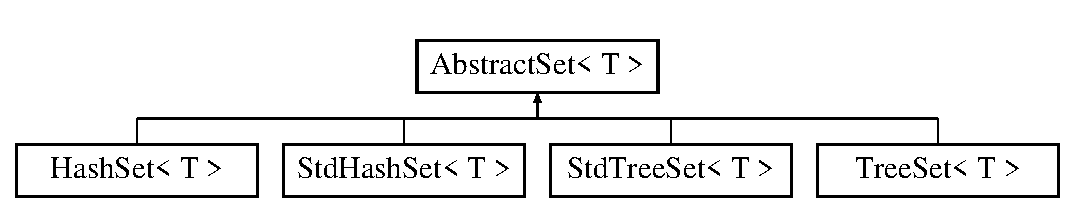
\includegraphics[height=2.000000cm]{class_abstract_set}
\end{center}
\end{figure}
\subsection*{Public Member Functions}
\begin{DoxyCompactItemize}
\item 
\hypertarget{class_abstract_set_a8306cfe855dc733b25a91ae030fe815a}{virtual \hyperlink{class_abstract_set_a8306cfe855dc733b25a91ae030fe815a}{$\sim$\-Abstract\-Set} ()}\label{class_abstract_set_a8306cfe855dc733b25a91ae030fe815a}

\begin{DoxyCompactList}\small\item\em Destructor for the set. \end{DoxyCompactList}\item 
\hypertarget{class_abstract_set_ad7e6f3001d69f7c12e1890585aabf76b}{virtual size\-\_\-t \hyperlink{class_abstract_set_ad7e6f3001d69f7c12e1890585aabf76b}{size} () const =0}\label{class_abstract_set_ad7e6f3001d69f7c12e1890585aabf76b}

\begin{DoxyCompactList}\small\item\em Size of the set. \end{DoxyCompactList}\item 
\hypertarget{class_abstract_set_a12afe4c5cea823491fdfca02cc644bf3}{virtual void \hyperlink{class_abstract_set_a12afe4c5cea823491fdfca02cc644bf3}{insert} (const T \&x)=0}\label{class_abstract_set_a12afe4c5cea823491fdfca02cc644bf3}

\begin{DoxyCompactList}\small\item\em Inserts an element into the set. \end{DoxyCompactList}\item 
\hypertarget{class_abstract_set_a2b9d1b3662218ab3ba98fd3db085852f}{virtual bool \hyperlink{class_abstract_set_a2b9d1b3662218ab3ba98fd3db085852f}{exists} (const T \&x) const =0}\label{class_abstract_set_a2b9d1b3662218ab3ba98fd3db085852f}

\begin{DoxyCompactList}\small\item\em Checks if the element is in the set. \end{DoxyCompactList}\item 
\hypertarget{class_abstract_set_a60770781af640d8060abac15f14e3d2e}{virtual void \hyperlink{class_abstract_set_a60770781af640d8060abac15f14e3d2e}{debug} () const =0}\label{class_abstract_set_a60770781af640d8060abac15f14e3d2e}

\begin{DoxyCompactList}\small\item\em Prints debugging information to cerr. \end{DoxyCompactList}\end{DoxyCompactItemize}


\subsection{Detailed Description}
\subsubsection*{template$<$typename T$>$class Abstract\-Set$<$ T $>$}

\hyperlink{class_abstract_set}{Abstract\-Set} to be inherited. 

The documentation for this class was generated from the following file\-:\begin{DoxyCompactItemize}
\item 
\hyperlink{abstractset_8hpp}{abstractset.\-hpp}\end{DoxyCompactItemize}

\hypertarget{class_cow}{\section{Cow Class Reference}
\label{class_cow}\index{Cow@{Cow}}
}


Test class which implements the bare minimum to be usable with the sets.  


\subsection*{Public Member Functions}
\begin{DoxyCompactItemize}
\item 
\hypertarget{class_cow_a7d60406c5ed4761cf6e71c329762255f}{\hyperlink{class_cow_a7d60406c5ed4761cf6e71c329762255f}{Cow} (size\-\_\-t num\-Hats)}\label{class_cow_a7d60406c5ed4761cf6e71c329762255f}

\begin{DoxyCompactList}\small\item\em Non-\/default constructor. \end{DoxyCompactList}\end{DoxyCompactItemize}
\subsection*{Friends}
\begin{DoxyCompactItemize}
\item 
\hypertarget{class_cow_a23e10f6dc9387f62836b1a11290f7432}{std\-::ostream \& \hyperlink{class_cow_a23e10f6dc9387f62836b1a11290f7432}{operator$<$$<$} (std\-::ostream \&out, const \hyperlink{class_cow}{Cow} \&print\-Me)}\label{class_cow_a23e10f6dc9387f62836b1a11290f7432}

\begin{DoxyCompactList}\small\item\em Output a \hyperlink{class_cow}{Cow} in visual form. \end{DoxyCompactList}\item 
\hypertarget{class_cow_ad9b4faa3b4ff57053311dfc10dc65bf1}{bool \hyperlink{class_cow_ad9b4faa3b4ff57053311dfc10dc65bf1}{operator$<$} (const \hyperlink{class_cow}{Cow} \&lhs, const \hyperlink{class_cow}{Cow} \&rhs)}\label{class_cow_ad9b4faa3b4ff57053311dfc10dc65bf1}

\begin{DoxyCompactList}\small\item\em Inequality for Cows. \end{DoxyCompactList}\end{DoxyCompactItemize}


\subsection{Detailed Description}
Test class which implements the bare minimum to be usable with the sets. 

\begin{DoxyRemark}{Remarks}
As this class is very brief and intended purely for testing purposes, we keep it completely contained within this file. Doing so on production level code is problematic. 
\end{DoxyRemark}


The documentation for this class was generated from the following file\-:\begin{DoxyCompactItemize}
\item 
generic-\/set-\/tests.\-cpp\end{DoxyCompactItemize}

\hypertarget{class_hash_set_1_1_element}{\section{Hash\-Set$<$ T $>$\-:\-:Element Class Reference}
\label{class_hash_set_1_1_element}\index{Hash\-Set$<$ T $>$\-::\-Element@{Hash\-Set$<$ T $>$\-::\-Element}}
}


Array of Elements.  


\subsection*{Public Attributes}
\begin{DoxyCompactItemize}
\item 
\hypertarget{class_hash_set_1_1_element_a6245ad05cf796ac9330c8eea0d50aa2a}{const T $\ast$ {\bfseries data\-\_\-}}\label{class_hash_set_1_1_element_a6245ad05cf796ac9330c8eea0d50aa2a}

\item 
\hypertarget{class_hash_set_1_1_element_ad54392827ded611f0734b6346f3da14f}{bool {\bfseries used\-\_\-}}\label{class_hash_set_1_1_element_ad54392827ded611f0734b6346f3da14f}

\end{DoxyCompactItemize}


\subsection{Detailed Description}
\subsubsection*{template$<$typename T$>$class Hash\-Set$<$ T $>$\-::\-Element}

Array of Elements. 

Stores a constant pointer of type T, and a boolean that checks if the element has been included in the hash.

This class uses a pointer to type T since we do not want to change it. 

The documentation for this class was generated from the following file\-:\begin{DoxyCompactItemize}
\item 
\hyperlink{hashset_8hpp}{hashset.\-hpp}\end{DoxyCompactItemize}

\hypertarget{class_hash_set}{\section{Hash\-Set$<$ T $>$ Class Template Reference}
\label{class_hash_set}\index{Hash\-Set$<$ T $>$@{Hash\-Set$<$ T $>$}}
}


Hashset for an arbitrary class T.  




{\ttfamily \#include $<$hashset.\-hpp$>$}

Inheritance diagram for Hash\-Set$<$ T $>$\-:\begin{figure}[H]
\begin{center}
\leavevmode
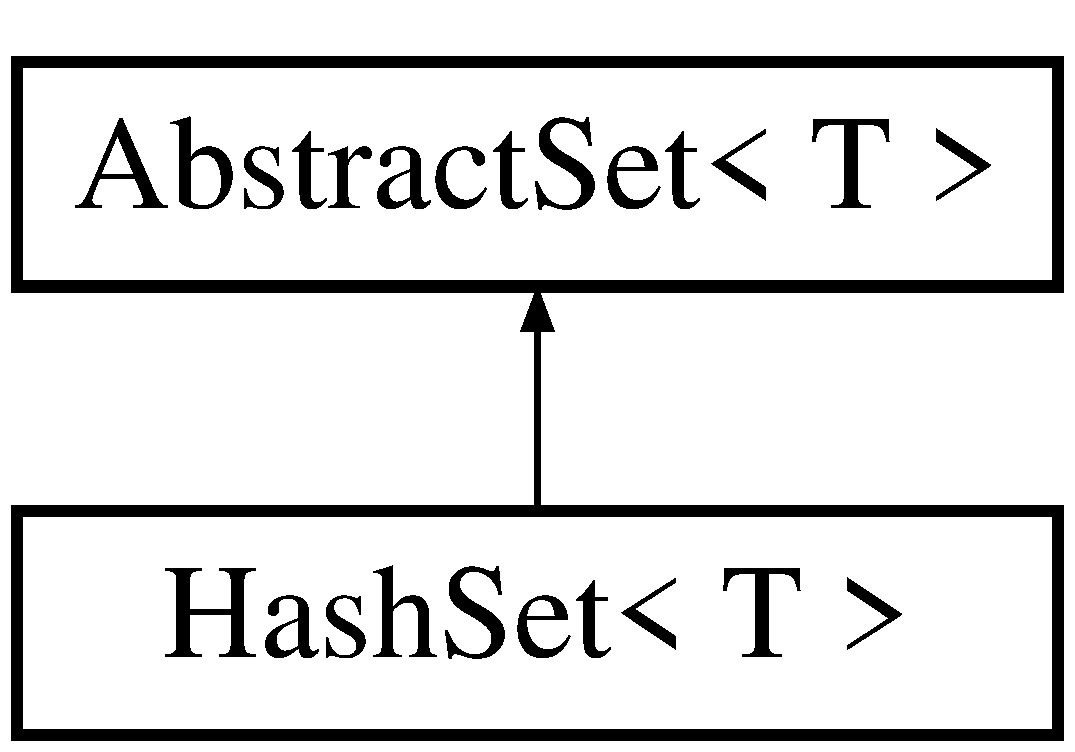
\includegraphics[height=2.000000cm]{class_hash_set}
\end{center}
\end{figure}
\subsection*{Classes}
\begin{DoxyCompactItemize}
\item 
class \hyperlink{class_hash_set_1_1_element}{Element}
\begin{DoxyCompactList}\small\item\em Array of Elements. \end{DoxyCompactList}\end{DoxyCompactItemize}
\subsection*{Public Member Functions}
\begin{DoxyCompactItemize}
\item 
\hyperlink{class_hash_set_af3813c169024060da2044aafe3851a8d}{Hash\-Set} ()
\begin{DoxyCompactList}\small\item\em Default constructor for \hyperlink{class_hash_set}{Hash\-Set}. \end{DoxyCompactList}\item 
\hypertarget{class_hash_set_a58686b84c9bb5e744e279e5d52b8c656}{\hyperlink{class_hash_set_a58686b84c9bb5e744e279e5d52b8c656}{$\sim$\-Hash\-Set} ()}\label{class_hash_set_a58686b84c9bb5e744e279e5d52b8c656}

\begin{DoxyCompactList}\small\item\em Returns the number of objects stored in the hash. \end{DoxyCompactList}\item 
\hypertarget{class_hash_set_a50921b9d5cacac394dc71a63bee037a7}{size\-\_\-t \hyperlink{class_hash_set_a50921b9d5cacac394dc71a63bee037a7}{size} () const }\label{class_hash_set_a50921b9d5cacac394dc71a63bee037a7}

\begin{DoxyCompactList}\small\item\em Size of the set. \end{DoxyCompactList}\item 
void \hyperlink{class_hash_set_a0134587851696ec3f2cb41c34f7f70b5}{insert} (const T \&x)
\begin{DoxyCompactList}\small\item\em Inserts the object of type T into the hash. \end{DoxyCompactList}\item 
bool \hyperlink{class_hash_set_a791fc527424c724a415ebd88b38a42ba}{exists} (const T \&x) const 
\begin{DoxyCompactList}\small\item\em Checks if the object of type T is in the hash. \end{DoxyCompactList}\item 
\hypertarget{class_hash_set_a549b200c4b34ef30b8dafbbae6cad008}{size\-\_\-t \hyperlink{class_hash_set_a549b200c4b34ef30b8dafbbae6cad008}{buckets} () const }\label{class_hash_set_a549b200c4b34ef30b8dafbbae6cad008}

\begin{DoxyCompactList}\small\item\em Returns the number of buckets. \end{DoxyCompactList}\item 
\hypertarget{class_hash_set_a85c4d8f088f5679d587e06c07c362ac5}{size\-\_\-t \hyperlink{class_hash_set_a85c4d8f088f5679d587e06c07c362ac5}{reallocations} () const }\label{class_hash_set_a85c4d8f088f5679d587e06c07c362ac5}

\begin{DoxyCompactList}\small\item\em Returns the number of times the hash table has resized itself. \end{DoxyCompactList}\item 
size\-\_\-t \hyperlink{class_hash_set_a54fa80d8af72e633479aa4520a7e5d2f}{collisions} () const 
\item 
size\-\_\-t \hyperlink{class_hash_set_a21daebf2846f630ab4300c4c0468c929}{maximal} () const 
\item 
\hypertarget{class_hash_set_a83defc0197ac5362971ff18a210205f6}{void \hyperlink{class_hash_set_a83defc0197ac5362971ff18a210205f6}{debug} () const }\label{class_hash_set_a83defc0197ac5362971ff18a210205f6}

\begin{DoxyCompactList}\small\item\em Prints debugging information for the \hyperlink{class_hash_set}{Hash\-Set} to cerr. \end{DoxyCompactList}\end{DoxyCompactItemize}
\subsection*{Private Member Functions}
\begin{DoxyCompactItemize}
\item 
\hypertarget{class_hash_set_a7058a76053ccf7b2955e416e44365cf9}{\hyperlink{class_hash_set_a7058a76053ccf7b2955e416e44365cf9}{Hash\-Set} (size\-\_\-t capacity)}\label{class_hash_set_a7058a76053ccf7b2955e416e44365cf9}

\begin{DoxyCompactList}\small\item\em A constructor with a specific bucket size. \end{DoxyCompactList}\item 
void \hyperlink{class_hash_set_ae3040dd5da7885460b5b88469e9ecded}{rehash} (size\-\_\-t capacity)
\begin{DoxyCompactList}\small\item\em Makes a new hash size a given capacity. \end{DoxyCompactList}\end{DoxyCompactItemize}
\subsection*{Private Attributes}
\begin{DoxyCompactItemize}
\item 
\hypertarget{class_hash_set_a48e5037452fe348a0158bc458a75addf}{\hyperlink{class_hash_set_1_1_element}{Element} $\ast$ {\bfseries hash\-Table\-\_\-}}\label{class_hash_set_a48e5037452fe348a0158bc458a75addf}

\item 
\hypertarget{class_hash_set_a927cc07bbfc932aaaa985b50990d4126}{size\-\_\-t \hyperlink{class_hash_set_a927cc07bbfc932aaaa985b50990d4126}{size\-\_\-}}\label{class_hash_set_a927cc07bbfc932aaaa985b50990d4126}

\begin{DoxyCompactList}\small\item\em The number of objects in the hash. \end{DoxyCompactList}\item 
\hypertarget{class_hash_set_a929b2d9417ba1cdff9577d4f0357810e}{size\-\_\-t \hyperlink{class_hash_set_a929b2d9417ba1cdff9577d4f0357810e}{buckets\-\_\-}}\label{class_hash_set_a929b2d9417ba1cdff9577d4f0357810e}

\begin{DoxyCompactList}\small\item\em The number of buckets. \end{DoxyCompactList}\item 
\hypertarget{class_hash_set_a70a507309fe986092691a68fb7d006ad}{size\-\_\-t \hyperlink{class_hash_set_a70a507309fe986092691a68fb7d006ad}{reallocations\-\_\-}}\label{class_hash_set_a70a507309fe986092691a68fb7d006ad}

\begin{DoxyCompactList}\small\item\em The number of reallocations. \end{DoxyCompactList}\item 
\hypertarget{class_hash_set_acc755fe1139cf94e303c9b3c98ea3c35}{size\-\_\-t \hyperlink{class_hash_set_acc755fe1139cf94e303c9b3c98ea3c35}{collisions\-\_\-}}\label{class_hash_set_acc755fe1139cf94e303c9b3c98ea3c35}

\begin{DoxyCompactList}\small\item\em The number of collisions. \end{DoxyCompactList}\item 
\hypertarget{class_hash_set_af3d4c11d45397596369b76c964382888}{size\-\_\-t \hyperlink{class_hash_set_af3d4c11d45397596369b76c964382888}{maximal\-\_\-}}\label{class_hash_set_af3d4c11d45397596369b76c964382888}

\begin{DoxyCompactList}\small\item\em The length of the longest chain. \end{DoxyCompactList}\end{DoxyCompactItemize}
\subsection*{Static Private Attributes}
\begin{DoxyCompactItemize}
\item 
static const double \hyperlink{class_hash_set_a0d5b0c2205b8b785733e0f71048af858}{L\-O\-A\-D\-\_\-\-F\-A\-C\-T\-O\-R} = 0.\-5
\item 
\hypertarget{class_hash_set_a66c7bc6922aa4d11ba69cad985da45f3}{static const size\-\_\-t {\bfseries R\-E\-S\-I\-Z\-E\-\_\-\-F\-A\-C\-T\-O\-R} = 2}\label{class_hash_set_a66c7bc6922aa4d11ba69cad985da45f3}

\end{DoxyCompactItemize}


\subsection{Detailed Description}
\subsubsection*{template$<$typename T$>$class Hash\-Set$<$ T $>$}

Hashset for an arbitrary class T. 

This class includes a class \hyperlink{class_hash_set_1_1_element}{Element} that has data members that holds a pointer to a T type object called data\-\_\- and a boolean called used\-\_\- that shows if the \hyperlink{class_hash_set_1_1_element}{Element} has been inserted into the hash.

\begin{DoxyRemark}{Remarks}
Deletion is not supported. 
\end{DoxyRemark}


\subsection{Constructor \& Destructor Documentation}
\hypertarget{class_hash_set_af3813c169024060da2044aafe3851a8d}{\index{Hash\-Set@{Hash\-Set}!Hash\-Set@{Hash\-Set}}
\index{Hash\-Set@{Hash\-Set}!HashSet@{Hash\-Set}}
\subsubsection[{Hash\-Set}]{\setlength{\rightskip}{0pt plus 5cm}template$<$typename T $>$ {\bf Hash\-Set}$<$ T $>$\-::{\bf Hash\-Set} (
\begin{DoxyParamCaption}
{}
\end{DoxyParamCaption}
)}}\label{class_hash_set_af3813c169024060da2044aafe3851a8d}


Default constructor for \hyperlink{class_hash_set}{Hash\-Set}. 

Initializes buckets\-\_\- as 2 and the remaining data members as 0. All Elements are initialized as false for used\-\_\-.\-Destructor. Deletes the pointers. 

\subsection{Member Function Documentation}
\hypertarget{class_hash_set_a54fa80d8af72e633479aa4520a7e5d2f}{\index{Hash\-Set@{Hash\-Set}!collisions@{collisions}}
\index{collisions@{collisions}!HashSet@{Hash\-Set}}
\subsubsection[{collisions}]{\setlength{\rightskip}{0pt plus 5cm}template$<$typename T $>$ size\-\_\-t {\bf Hash\-Set}$<$ T $>$\-::collisions (
\begin{DoxyParamCaption}
{}
\end{DoxyParamCaption}
) const}}\label{class_hash_set_a54fa80d8af72e633479aa4520a7e5d2f}
Returns that number of times an insert into the current hash table representation has found a non-\/empty bucket. \hypertarget{class_hash_set_a791fc527424c724a415ebd88b38a42ba}{\index{Hash\-Set@{Hash\-Set}!exists@{exists}}
\index{exists@{exists}!HashSet@{Hash\-Set}}
\subsubsection[{exists}]{\setlength{\rightskip}{0pt plus 5cm}template$<$typename T $>$ bool {\bf Hash\-Set}$<$ T $>$\-::exists (
\begin{DoxyParamCaption}
\item[{const T \&}]{x}
\end{DoxyParamCaption}
) const\hspace{0.3cm}{\ttfamily [virtual]}}}\label{class_hash_set_a791fc527424c724a415ebd88b38a42ba}


Checks if the object of type T is in the hash. 


\begin{DoxyParams}{Parameters}
{\em x} & A reference to a constant T. \\
\hline
\end{DoxyParams}


Implements \hyperlink{class_abstract_set_a2b9d1b3662218ab3ba98fd3db085852f}{Abstract\-Set$<$ T $>$}.

\hypertarget{class_hash_set_a0134587851696ec3f2cb41c34f7f70b5}{\index{Hash\-Set@{Hash\-Set}!insert@{insert}}
\index{insert@{insert}!HashSet@{Hash\-Set}}
\subsubsection[{insert}]{\setlength{\rightskip}{0pt plus 5cm}template$<$typename T $>$ void {\bf Hash\-Set}$<$ T $>$\-::insert (
\begin{DoxyParamCaption}
\item[{const T \&}]{x}
\end{DoxyParamCaption}
)\hspace{0.3cm}{\ttfamily [virtual]}}}\label{class_hash_set_a0134587851696ec3f2cb41c34f7f70b5}


Inserts the object of type T into the hash. 

Insert will cause the hash to resize itself when size\-\_\-/buckets\-\_\- is greater than the load factor.


\begin{DoxyParams}{Parameters}
{\em x} & A reference to a constant T. \\
\hline
\end{DoxyParams}


Implements \hyperlink{class_abstract_set_a12afe4c5cea823491fdfca02cc644bf3}{Abstract\-Set$<$ T $>$}.

\hypertarget{class_hash_set_a21daebf2846f630ab4300c4c0468c929}{\index{Hash\-Set@{Hash\-Set}!maximal@{maximal}}
\index{maximal@{maximal}!HashSet@{Hash\-Set}}
\subsubsection[{maximal}]{\setlength{\rightskip}{0pt plus 5cm}template$<$typename T $>$ size\-\_\-t {\bf Hash\-Set}$<$ T $>$\-::maximal (
\begin{DoxyParamCaption}
{}
\end{DoxyParamCaption}
) const}}\label{class_hash_set_a21daebf2846f630ab4300c4c0468c929}
Returns the length of the longest chain (in the case of separate chaining) or cluster (in the case of open addressing) discovered so far in the current hash table representation. \hypertarget{class_hash_set_ae3040dd5da7885460b5b88469e9ecded}{\index{Hash\-Set@{Hash\-Set}!rehash@{rehash}}
\index{rehash@{rehash}!HashSet@{Hash\-Set}}
\subsubsection[{rehash}]{\setlength{\rightskip}{0pt plus 5cm}template$<$typename T $>$ void {\bf Hash\-Set}$<$ T $>$\-::rehash (
\begin{DoxyParamCaption}
\item[{size\-\_\-t}]{capacity}
\end{DoxyParamCaption}
)\hspace{0.3cm}{\ttfamily [private]}}}\label{class_hash_set_ae3040dd5da7885460b5b88469e9ecded}


Makes a new hash size a given capacity. 


\begin{DoxyParams}{Parameters}
{\em capacity} & The number of buckets that the new hash will have. \\
\hline
\end{DoxyParams}


\subsection{Member Data Documentation}
\hypertarget{class_hash_set_a0d5b0c2205b8b785733e0f71048af858}{\index{Hash\-Set@{Hash\-Set}!L\-O\-A\-D\-\_\-\-F\-A\-C\-T\-O\-R@{L\-O\-A\-D\-\_\-\-F\-A\-C\-T\-O\-R}}
\index{L\-O\-A\-D\-\_\-\-F\-A\-C\-T\-O\-R@{L\-O\-A\-D\-\_\-\-F\-A\-C\-T\-O\-R}!HashSet@{Hash\-Set}}
\subsubsection[{L\-O\-A\-D\-\_\-\-F\-A\-C\-T\-O\-R}]{\setlength{\rightskip}{0pt plus 5cm}template$<$typename T$>$ const double {\bf Hash\-Set}$<$ T $>$\-::L\-O\-A\-D\-\_\-\-F\-A\-C\-T\-O\-R = 0.\-5\hspace{0.3cm}{\ttfamily [static]}, {\ttfamily [private]}}}\label{class_hash_set_a0d5b0c2205b8b785733e0f71048af858}
We used a simple 50\% load factor, which seemed to be sufficient to keep overhead reasonable while not undermining our assumption of constant amortized time. 

The documentation for this class was generated from the following files\-:\begin{DoxyCompactItemize}
\item 
\hyperlink{hashset_8hpp}{hashset.\-hpp}\item 
\hyperlink{hashset-private_8hpp}{hashset-\/private.\-hpp}\end{DoxyCompactItemize}

\hypertarget{class_std_hash_set_1_1_my_hash}{\section{Std\-Hash\-Set$<$ T $>$\-:\-:My\-Hash Class Reference}
\label{class_std_hash_set_1_1_my_hash}\index{Std\-Hash\-Set$<$ T $>$\-::\-My\-Hash@{Std\-Hash\-Set$<$ T $>$\-::\-My\-Hash}}
}
\subsection*{Public Member Functions}
\begin{DoxyCompactItemize}
\item 
\hypertarget{class_std_hash_set_1_1_my_hash_aac2096f95c7a7bd613cfb4a65d1d09e7}{size\-\_\-t {\bfseries operator()} (const T \&value) const }\label{class_std_hash_set_1_1_my_hash_aac2096f95c7a7bd613cfb4a65d1d09e7}

\end{DoxyCompactItemize}


The documentation for this class was generated from the following file\-:\begin{DoxyCompactItemize}
\item 
\hyperlink{stdhashset_8hpp}{stdhashset.\-hpp}\end{DoxyCompactItemize}

\hypertarget{class_tree_set_1_1_node}{\section{Tree\-Set$<$ T $>$\-:\-:Node Class Reference}
\label{class_tree_set_1_1_node}\index{Tree\-Set$<$ T $>$\-::\-Node@{Tree\-Set$<$ T $>$\-::\-Node}}
}


Class that stores information about an element in the tree.  


\subsection*{Public Member Functions}
\begin{DoxyCompactItemize}
\item 
\hypertarget{class_tree_set_1_1_node_aa1cc5ccf4ccd83cef2cce3c4e997b809}{{\bfseries Node} (const T \&x)}\label{class_tree_set_1_1_node_aa1cc5ccf4ccd83cef2cce3c4e997b809}

\item 
\hypertarget{class_tree_set_1_1_node_a4e4ac47b0a96808448280fb9b7331030}{\hyperlink{class_tree_set_1_1_node_a4e4ac47b0a96808448280fb9b7331030}{$\sim$\-Node} ()}\label{class_tree_set_1_1_node_a4e4ac47b0a96808448280fb9b7331030}

\begin{DoxyCompactList}\small\item\em Recursively deletes subtrees. \end{DoxyCompactList}\end{DoxyCompactItemize}
\subsection*{Public Attributes}
\begin{DoxyCompactItemize}
\item 
\hypertarget{class_tree_set_1_1_node_a6617530db02b2548423f9e509ea48800}{T {\bfseries value\-\_\-}}\label{class_tree_set_1_1_node_a6617530db02b2548423f9e509ea48800}

\item 
\hypertarget{class_tree_set_1_1_node_a39e0fcfe30ba521c400734a2acdfe59c}{\hyperlink{class_tree_set_1_1_node}{Node} $\ast$ {\bfseries left\-\_\-}}\label{class_tree_set_1_1_node_a39e0fcfe30ba521c400734a2acdfe59c}

\item 
\hypertarget{class_tree_set_1_1_node_a4fac1f38c4727f108cdc732224afc34c}{\hyperlink{class_tree_set_1_1_node}{Node} $\ast$ {\bfseries right\-\_\-}}\label{class_tree_set_1_1_node_a4fac1f38c4727f108cdc732224afc34c}

\item 
\hypertarget{class_tree_set_1_1_node_a717d750139268bc9b2f8f1994c42efa1}{int {\bfseries height\-\_\-}}\label{class_tree_set_1_1_node_a717d750139268bc9b2f8f1994c42efa1}

\end{DoxyCompactItemize}


\subsection{Detailed Description}
\subsubsection*{template$<$typename T$>$class Tree\-Set$<$ T $>$\-::\-Node}

Class that stores information about an element in the tree. 

Because it is an A\-V\-L tree, each node keeps track of its own height. Contains pointers to the root nodes of the left and right subtrees. 

The documentation for this class was generated from the following files\-:\begin{DoxyCompactItemize}
\item 
\hyperlink{treeset_8hpp}{treeset.\-hpp}\item 
\hyperlink{treeset-private_8hpp}{treeset-\/private.\-hpp}\end{DoxyCompactItemize}

\hypertarget{class_std_hash_set}{\section{Std\-Hash\-Set$<$ T $>$ Class Template Reference}
\label{class_std_hash_set}\index{Std\-Hash\-Set$<$ T $>$@{Std\-Hash\-Set$<$ T $>$}}
}


Wrapper class for S\-T\-L unordered\-\_\-set.  




{\ttfamily \#include $<$stdhashset.\-hpp$>$}

Inheritance diagram for Std\-Hash\-Set$<$ T $>$\-:\begin{figure}[H]
\begin{center}
\leavevmode
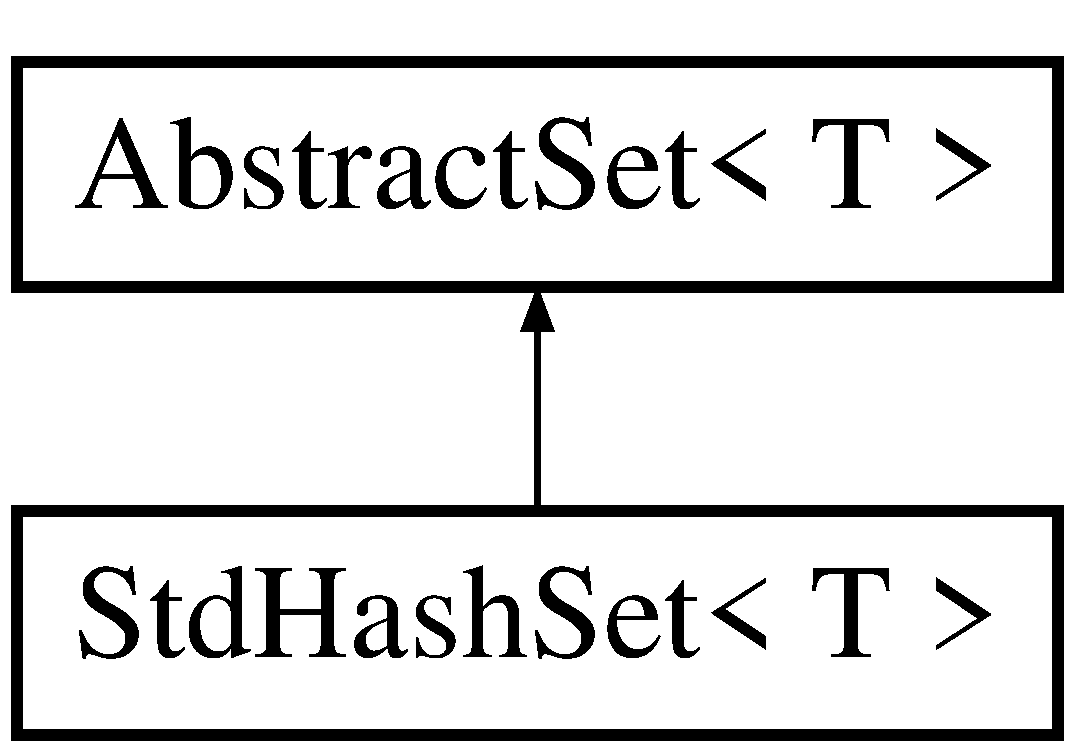
\includegraphics[height=2.000000cm]{class_std_hash_set}
\end{center}
\end{figure}
\subsection*{Classes}
\begin{DoxyCompactItemize}
\item 
class \hyperlink{class_std_hash_set_1_1_my_hash}{My\-Hash}
\end{DoxyCompactItemize}
\subsection*{Public Member Functions}
\begin{DoxyCompactItemize}
\item 
\hypertarget{class_std_hash_set_a663408a739a42a3f2b5e74e4097a354a}{size\-\_\-t \hyperlink{class_std_hash_set_a663408a739a42a3f2b5e74e4097a354a}{size} () const }\label{class_std_hash_set_a663408a739a42a3f2b5e74e4097a354a}

\begin{DoxyCompactList}\small\item\em Returns the number of objects stored in the set. \end{DoxyCompactList}\item 
\hypertarget{class_std_hash_set_a4e39ef224e2ee7d1c065c7f50e71aad5}{void \hyperlink{class_std_hash_set_a4e39ef224e2ee7d1c065c7f50e71aad5}{insert} (const T \&x)}\label{class_std_hash_set_a4e39ef224e2ee7d1c065c7f50e71aad5}

\begin{DoxyCompactList}\small\item\em Inserts the element into the set. \end{DoxyCompactList}\item 
\hypertarget{class_std_hash_set_a54040efb148792c1317ea6f892222a61}{bool \hyperlink{class_std_hash_set_a54040efb148792c1317ea6f892222a61}{exists} (const T \&x) const }\label{class_std_hash_set_a54040efb148792c1317ea6f892222a61}

\begin{DoxyCompactList}\small\item\em Determines whether the element is in the set. \end{DoxyCompactList}\item 
\hypertarget{class_std_hash_set_a23a35f0c0204e06b8dfa8becfab5fdfb}{void \hyperlink{class_std_hash_set_a23a35f0c0204e06b8dfa8becfab5fdfb}{debug} () const }\label{class_std_hash_set_a23a35f0c0204e06b8dfa8becfab5fdfb}

\begin{DoxyCompactList}\small\item\em Prints the debugging information to cerr. \end{DoxyCompactList}\end{DoxyCompactItemize}
\subsection*{Private Attributes}
\begin{DoxyCompactItemize}
\item 
\hypertarget{class_std_hash_set_ab4227f337aa0f9b76b1cd855ecdc8929}{std\-::unordered\-\_\-set$<$ T, \hyperlink{class_std_hash_set_1_1_my_hash}{My\-Hash} $>$ {\bfseries hash\-Set\-\_\-}}\label{class_std_hash_set_ab4227f337aa0f9b76b1cd855ecdc8929}

\end{DoxyCompactItemize}


\subsection{Detailed Description}
\subsubsection*{template$<$typename T$>$class Std\-Hash\-Set$<$ T $>$}

Wrapper class for S\-T\-L unordered\-\_\-set. 

Compiler synthesized constructor and destructor are adequate. 

The documentation for this class was generated from the following files\-:\begin{DoxyCompactItemize}
\item 
\hyperlink{stdhashset_8hpp}{stdhashset.\-hpp}\item 
\hyperlink{stdhashset-private_8hpp}{stdhashset-\/private.\-hpp}\end{DoxyCompactItemize}

\hypertarget{class_std_tree_set}{\section{Std\-Tree\-Set$<$ T $>$ Class Template Reference}
\label{class_std_tree_set}\index{Std\-Tree\-Set$<$ T $>$@{Std\-Tree\-Set$<$ T $>$}}
}


Wrapper class for S\-T\-L set.  




{\ttfamily \#include $<$stdtreeset.\-hpp$>$}

Inheritance diagram for Std\-Tree\-Set$<$ T $>$\-:\begin{figure}[H]
\begin{center}
\leavevmode
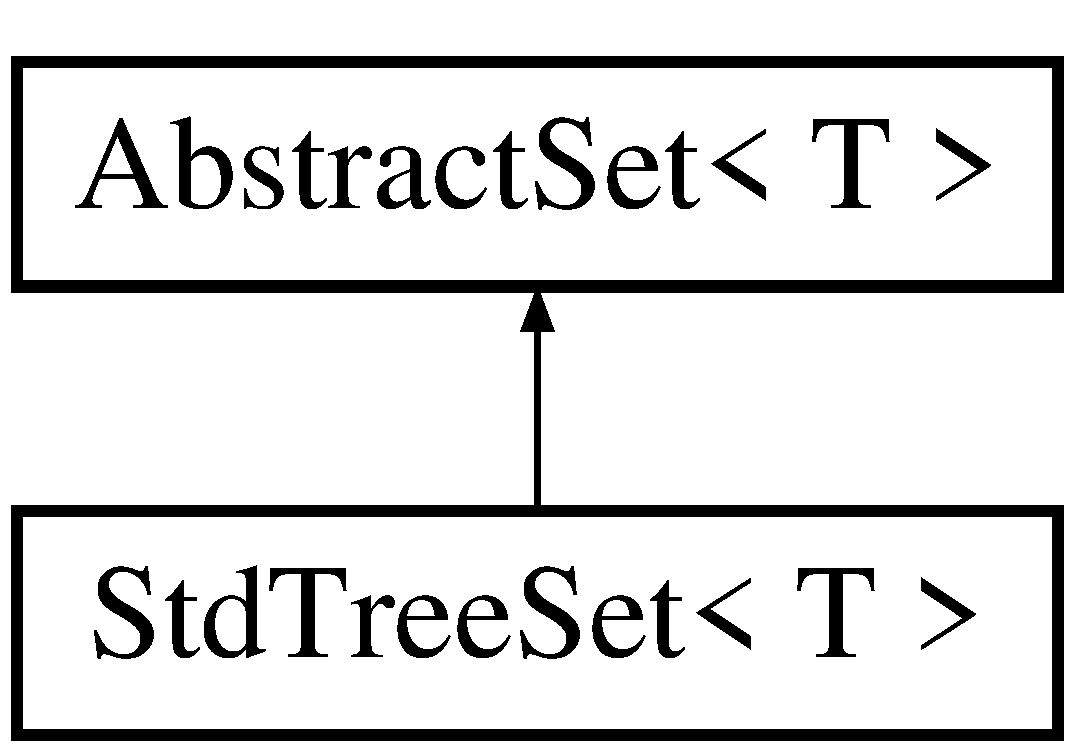
\includegraphics[height=2.000000cm]{class_std_tree_set}
\end{center}
\end{figure}
\subsection*{Public Member Functions}
\begin{DoxyCompactItemize}
\item 
\hypertarget{class_std_tree_set_a842965914d664c4038d2686fbdc674ac}{size\-\_\-t \hyperlink{class_std_tree_set_a842965914d664c4038d2686fbdc674ac}{size} () const }\label{class_std_tree_set_a842965914d664c4038d2686fbdc674ac}

\begin{DoxyCompactList}\small\item\em Returns the number of objects stored in the set. \end{DoxyCompactList}\item 
\hypertarget{class_std_tree_set_aba8ab0c22468935472982b48e6eeef46}{void \hyperlink{class_std_tree_set_aba8ab0c22468935472982b48e6eeef46}{insert} (const T \&x)}\label{class_std_tree_set_aba8ab0c22468935472982b48e6eeef46}

\begin{DoxyCompactList}\small\item\em Inserts the element into the set. \end{DoxyCompactList}\item 
\hypertarget{class_std_tree_set_a6cb54379f9ebbc21162bd50fcb1a40d6}{bool \hyperlink{class_std_tree_set_a6cb54379f9ebbc21162bd50fcb1a40d6}{exists} (const T \&x) const }\label{class_std_tree_set_a6cb54379f9ebbc21162bd50fcb1a40d6}

\begin{DoxyCompactList}\small\item\em Determines whether the element is in the set. \end{DoxyCompactList}\item 
\hypertarget{class_std_tree_set_aece05dc24990b35f85de36087345556c}{void \hyperlink{class_std_tree_set_aece05dc24990b35f85de36087345556c}{debug} () const }\label{class_std_tree_set_aece05dc24990b35f85de36087345556c}

\begin{DoxyCompactList}\small\item\em Prints the debugging information to cerr. \end{DoxyCompactList}\end{DoxyCompactItemize}


\subsection{Detailed Description}
\subsubsection*{template$<$typename T$>$class Std\-Tree\-Set$<$ T $>$}

Wrapper class for S\-T\-L set. 

Compiler synthesized constructor and destructor are adequate. 

The documentation for this class was generated from the following files\-:\begin{DoxyCompactItemize}
\item 
\hyperlink{stdtreeset_8hpp}{stdtreeset.\-hpp}\item 
\hyperlink{stdtreeset-private_8hpp}{stdtreeset-\/private.\-hpp}\end{DoxyCompactItemize}

\hypertarget{class_tree_set}{\section{Tree\-Set$<$ T $>$ Class Template Reference}
\label{class_tree_set}\index{Tree\-Set$<$ T $>$@{Tree\-Set$<$ T $>$}}
}


\hyperlink{class_tree_set}{Tree\-Set} to be inherited.  




{\ttfamily \#include $<$treeset.\-hpp$>$}

Inheritance diagram for Tree\-Set$<$ T $>$\-:\begin{figure}[H]
\begin{center}
\leavevmode
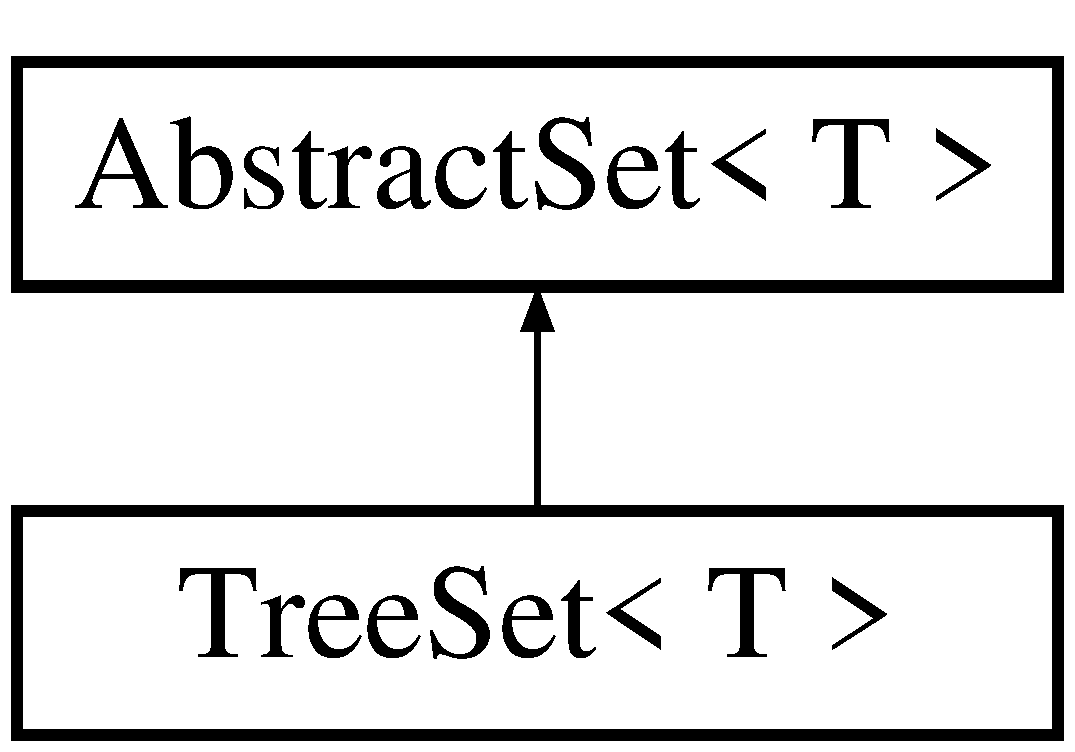
\includegraphics[height=2.000000cm]{class_tree_set}
\end{center}
\end{figure}
\subsection*{Public Member Functions}
\begin{DoxyCompactItemize}
\item 
\hypertarget{class_tree_set_a915f05820dc9f0e2ef34263f05951c6d}{\hyperlink{class_tree_set_a915f05820dc9f0e2ef34263f05951c6d}{Tree\-Set} ()}\label{class_tree_set_a915f05820dc9f0e2ef34263f05951c6d}

\begin{DoxyCompactList}\small\item\em Default constructor for \hyperlink{class_tree_set}{Tree\-Set}. \end{DoxyCompactList}\item 
\hyperlink{class_tree_set_a698f6c217e682f1ab29da87d89dd16b6}{$\sim$\-Tree\-Set} ()
\begin{DoxyCompactList}\small\item\em Destructor for \hyperlink{class_tree_set}{Tree\-Set}. \end{DoxyCompactList}\item 
\hypertarget{class_tree_set_ab8819494cda32c08cf9217f3419e4ff3}{size\-\_\-t \hyperlink{class_tree_set_ab8819494cda32c08cf9217f3419e4ff3}{size} () const }\label{class_tree_set_ab8819494cda32c08cf9217f3419e4ff3}

\begin{DoxyCompactList}\small\item\em Returns the number of objects stored in the tree. \end{DoxyCompactList}\item 
void \hyperlink{class_tree_set_a04a78c1b3d70968c6547589c8add3d4a}{insert} (const T \&x)
\begin{DoxyCompactList}\small\item\em Inserts an element into the tree. \end{DoxyCompactList}\item 
bool \hyperlink{class_tree_set_aee288e3b9299f8fcbac0834543865128}{exists} (const T \&x) const 
\begin{DoxyCompactList}\small\item\em Checks if the element exists in the tree. \end{DoxyCompactList}\item 
int \hyperlink{class_tree_set_a00da9efa0cac8a3dab15fd1c23e0d2b4}{height} () const 
\begin{DoxyCompactList}\small\item\em Returns the height of tree. \end{DoxyCompactList}\item 
\hypertarget{class_tree_set_af2af42baedbdf6d0d2a8b794f3a9eaa4}{std\-::ostream \& \hyperlink{class_tree_set_af2af42baedbdf6d0d2a8b794f3a9eaa4}{print} (std\-::ostream \&out) const }\label{class_tree_set_af2af42baedbdf6d0d2a8b794f3a9eaa4}

\begin{DoxyCompactList}\small\item\em Prints the tree. \end{DoxyCompactList}\item 
\hypertarget{class_tree_set_a05d9c633b020f9e759997f4ccb863ca2}{void \hyperlink{class_tree_set_a05d9c633b020f9e759997f4ccb863ca2}{debug} () const }\label{class_tree_set_a05d9c633b020f9e759997f4ccb863ca2}

\begin{DoxyCompactList}\small\item\em Prints debugging information for the \hyperlink{class_hash_set}{Hash\-Set} to cerr. \end{DoxyCompactList}\end{DoxyCompactItemize}


\subsection{Detailed Description}
\subsubsection*{template$<$typename T$>$class Tree\-Set$<$ T $>$}

\hyperlink{class_tree_set}{Tree\-Set} to be inherited. 

Uses an A\-V\-L Tree. 

\subsection{Constructor \& Destructor Documentation}
\hypertarget{class_tree_set_a698f6c217e682f1ab29da87d89dd16b6}{\index{Tree\-Set@{Tree\-Set}!$\sim$\-Tree\-Set@{$\sim$\-Tree\-Set}}
\index{$\sim$\-Tree\-Set@{$\sim$\-Tree\-Set}!TreeSet@{Tree\-Set}}
\subsubsection[{$\sim$\-Tree\-Set}]{\setlength{\rightskip}{0pt plus 5cm}template$<$typename T $>$ {\bf Tree\-Set}$<$ T $>$\-::$\sim${\bf Tree\-Set} (
\begin{DoxyParamCaption}
{}
\end{DoxyParamCaption}
)}}\label{class_tree_set_a698f6c217e682f1ab29da87d89dd16b6}


Destructor for \hyperlink{class_tree_set}{Tree\-Set}. 

Uses the destructor of the private class Node to recursively delete the tree. 

\subsection{Member Function Documentation}
\hypertarget{class_tree_set_aee288e3b9299f8fcbac0834543865128}{\index{Tree\-Set@{Tree\-Set}!exists@{exists}}
\index{exists@{exists}!TreeSet@{Tree\-Set}}
\subsubsection[{exists}]{\setlength{\rightskip}{0pt plus 5cm}template$<$typename T $>$ bool {\bf Tree\-Set}$<$ T $>$\-::exists (
\begin{DoxyParamCaption}
\item[{const T \&}]{x}
\end{DoxyParamCaption}
) const\hspace{0.3cm}{\ttfamily [virtual]}}}\label{class_tree_set_aee288e3b9299f8fcbac0834543865128}


Checks if the element exists in the tree. 

Calls a helper function to recursively search for the element. 

Implements \hyperlink{class_abstract_set_a2b9d1b3662218ab3ba98fd3db085852f}{Abstract\-Set$<$ T $>$}.

\hypertarget{class_tree_set_a00da9efa0cac8a3dab15fd1c23e0d2b4}{\index{Tree\-Set@{Tree\-Set}!height@{height}}
\index{height@{height}!TreeSet@{Tree\-Set}}
\subsubsection[{height}]{\setlength{\rightskip}{0pt plus 5cm}template$<$typename T $>$ int {\bf Tree\-Set}$<$ T $>$\-::height (
\begin{DoxyParamCaption}
{}
\end{DoxyParamCaption}
) const}}\label{class_tree_set_a00da9efa0cac8a3dab15fd1c23e0d2b4}


Returns the height of tree. 

Returns -\/1 for an empty tree. \hypertarget{class_tree_set_a04a78c1b3d70968c6547589c8add3d4a}{\index{Tree\-Set@{Tree\-Set}!insert@{insert}}
\index{insert@{insert}!TreeSet@{Tree\-Set}}
\subsubsection[{insert}]{\setlength{\rightskip}{0pt plus 5cm}template$<$typename T $>$ void {\bf Tree\-Set}$<$ T $>$\-::insert (
\begin{DoxyParamCaption}
\item[{const T \&}]{x}
\end{DoxyParamCaption}
)\hspace{0.3cm}{\ttfamily [virtual]}}}\label{class_tree_set_a04a78c1b3d70968c6547589c8add3d4a}


Inserts an element into the tree. 

Calls a helper function to recursively find the insertion point and balance the tree. 

Implements \hyperlink{class_abstract_set_a12afe4c5cea823491fdfca02cc644bf3}{Abstract\-Set$<$ T $>$}.



The documentation for this class was generated from the following files\-:\begin{DoxyCompactItemize}
\item 
\hyperlink{treeset_8hpp}{treeset.\-hpp}\item 
\hyperlink{treeset-private_8hpp}{treeset-\/private.\-hpp}\end{DoxyCompactItemize}

\chapter{File Documentation}
\hypertarget{abstractset_8hpp}{\section{abstractset.\-hpp File Reference}
\label{abstractset_8hpp}\index{abstractset.\-hpp@{abstractset.\-hpp}}
}


Abstract template \hyperlink{class_abstract_set}{Abstract\-Set} class.  


{\ttfamily \#include $<$ostream$>$}\\*
{\ttfamily \#include $<$cstddef$>$}\\*
\subsection*{Classes}
\begin{DoxyCompactItemize}
\item 
class \hyperlink{class_abstract_set}{Abstract\-Set$<$ T $>$}
\begin{DoxyCompactList}\small\item\em \hyperlink{class_abstract_set}{Abstract\-Set} to be inherited. \end{DoxyCompactList}\end{DoxyCompactItemize}


\subsection{Detailed Description}
Abstract template \hyperlink{class_abstract_set}{Abstract\-Set} class. \begin{DoxyAuthor}{Author}
Kevin Mc\-Swiggen and Mars Park 
\end{DoxyAuthor}

\hypertarget{hashset-private_8hpp}{\section{hashset-\/private.hpp File Reference}
\label{hashset-private_8hpp}\index{hashset-\/private.\-hpp@{hashset-\/private.\-hpp}}
}


The private implementation of the \hyperlink{class_hash_set}{Hash\-Set} template.  


{\ttfamily \#include $<$iostream$>$}\\*
{\ttfamily \#include $<$cstddef$>$}\\*
{\ttfamily \#include $<$algorithm$>$}\\*


\subsection{Detailed Description}
The private implementation of the \hyperlink{class_hash_set}{Hash\-Set} template. \begin{DoxyAuthor}{Author}
Kevin Mc\-Swiggen and Mars Park 
\end{DoxyAuthor}

\hypertarget{hashset_8hpp}{\section{hashset.\-hpp File Reference}
\label{hashset_8hpp}\index{hashset.\-hpp@{hashset.\-hpp}}
}


Declares the \hyperlink{class_hash_set}{Hash\-Set} class.  


{\ttfamily \#include $<$ostream$>$}\\*
{\ttfamily \#include $<$cstddef$>$}\\*
{\ttfamily \#include \char`\"{}abstractset.\-hpp\char`\"{}}\\*
{\ttfamily \#include \char`\"{}hashset-\/private.\-hpp\char`\"{}}\\*
\subsection*{Classes}
\begin{DoxyCompactItemize}
\item 
class \hyperlink{class_hash_set}{Hash\-Set$<$ T $>$}
\begin{DoxyCompactList}\small\item\em Hashset for an arbitrary class T. \end{DoxyCompactList}\end{DoxyCompactItemize}


\subsection{Detailed Description}
Declares the \hyperlink{class_hash_set}{Hash\-Set} class. \begin{DoxyAuthor}{Author}
Kevin Mc\-Swiggen and Mars Park 
\end{DoxyAuthor}

\hypertarget{myspell_8cpp}{\section{myspell.\-cpp File Reference}
\label{myspell_8cpp}\index{myspell.\-cpp@{myspell.\-cpp}}
}


Code for the My\-Spell spell checking program.  


{\ttfamily \#include \char`\"{}abstractset.\-hpp\char`\"{}}\\*
{\ttfamily \#include \char`\"{}stringhash.\-hpp\char`\"{}}\\*
{\ttfamily \#include \char`\"{}hashset.\-hpp\char`\"{}}\\*
{\ttfamily \#include \char`\"{}stdhashset.\-hpp\char`\"{}}\\*
{\ttfamily \#include \char`\"{}treeset.\-hpp\char`\"{}}\\*
{\ttfamily \#include \char`\"{}stdtreeset.\-hpp\char`\"{}}\\*
{\ttfamily \#include $<$iostream$>$}\\*
{\ttfamily \#include $<$fstream$>$}\\*
{\ttfamily \#include $<$cstddef$>$}\\*
{\ttfamily \#include $<$cstdlib$>$}\\*
{\ttfamily \#include $<$string$>$}\\*
{\ttfamily \#include $<$vector$>$}\\*
{\ttfamily \#include $<$list$>$}\\*
{\ttfamily \#include $<$cctype$>$}\\*
\subsection*{Functions}
\begin{DoxyCompactItemize}
\item 
void \hyperlink{myspell_8cpp_a1ff022344debd4323f3df7b0dabc088a}{usage} (const char $\ast$program\-Name)
\begin{DoxyCompactList}\small\item\em Print a usage message and exit. \end{DoxyCompactList}\item 
int \hyperlink{myspell_8cpp_acb02a6d171cf8bec5225d62422f18f36}{process\-Options} (int argc, const char $\ast$argv\mbox{[}$\,$\mbox{]}, bool \&debug, bool \&stdhash, bool \&ownhash, bool \&stdtree, bool \&owntree)
\begin{DoxyCompactList}\small\item\em Option processing. \end{DoxyCompactList}\item 
bool \hyperlink{myspell_8cpp_ac74592c006b1f8f15416598435dc6b5c}{read\-Dictionary} (const string \&file\-Name, \hyperlink{class_abstract_set}{Abstract\-Set}$<$ string $>$ $\ast$our\-Set)
\begin{DoxyCompactList}\small\item\em Generates a dictionary \hyperlink{class_abstract_set}{Abstract\-Set} for My\-Spell. \end{DoxyCompactList}\item 
void \hyperlink{myspell_8cpp_aaa408935628477487947e3820240bad5}{permute\-Spelling} (const string \&word, \hyperlink{class_abstract_set}{Abstract\-Set}$<$ string $>$ $\ast$dictionary)
\begin{DoxyCompactList}\small\item\em Helper function for check\-Spelling which generates suggestions. \end{DoxyCompactList}\item 
void \hyperlink{myspell_8cpp_a5470dc71d1982de0b3cad6312506a1fa}{check\-Spelling} (\hyperlink{class_abstract_set}{Abstract\-Set}$<$ string $>$ $\ast$dictionary, \hyperlink{class_abstract_set}{Abstract\-Set}$<$ string $>$ $\ast$seen)
\begin{DoxyCompactList}\small\item\em Checks input against an \hyperlink{class_abstract_set}{Abstract\-Set} dictionary of words. \end{DoxyCompactList}\item 
int \hyperlink{myspell_8cpp_ac0f2228420376f4db7e1274f2b41667c}{main} (int argc, const char $\ast$argv\mbox{[}$\,$\mbox{]})
\begin{DoxyCompactList}\small\item\em Main function for My\-Spell spellchecker. \end{DoxyCompactList}\end{DoxyCompactItemize}


\subsection{Detailed Description}
Code for the My\-Spell spell checking program. \begin{DoxyAuthor}{Author}
Kevin Mc\-Swiggen and Mars Park Option processing code adapted from Bailey Campbell's Nat\-Sel\-Path. 
\end{DoxyAuthor}


\subsection{Function Documentation}
\hypertarget{myspell_8cpp_a5470dc71d1982de0b3cad6312506a1fa}{\index{myspell.\-cpp@{myspell.\-cpp}!check\-Spelling@{check\-Spelling}}
\index{check\-Spelling@{check\-Spelling}!myspell.cpp@{myspell.\-cpp}}
\subsubsection[{check\-Spelling}]{\setlength{\rightskip}{0pt plus 5cm}void check\-Spelling (
\begin{DoxyParamCaption}
\item[{{\bf Abstract\-Set}$<$ string $>$ $\ast$}]{dictionary, }
\item[{{\bf Abstract\-Set}$<$ string $>$ $\ast$}]{seen}
\end{DoxyParamCaption}
)}}\label{myspell_8cpp_a5470dc71d1982de0b3cad6312506a1fa}


Checks input against an \hyperlink{class_abstract_set}{Abstract\-Set} dictionary of words. 

This function uses a previously-\/generated dictionary and compares input from cin against its content, offering spelling suggestions for any unrecognized words. \hypertarget{myspell_8cpp_ac0f2228420376f4db7e1274f2b41667c}{\index{myspell.\-cpp@{myspell.\-cpp}!main@{main}}
\index{main@{main}!myspell.cpp@{myspell.\-cpp}}
\subsubsection[{main}]{\setlength{\rightskip}{0pt plus 5cm}int main (
\begin{DoxyParamCaption}
\item[{int}]{argc, }
\item[{const char $\ast$}]{argv\mbox{[}$\,$\mbox{]}}
\end{DoxyParamCaption}
)}}\label{myspell_8cpp_ac0f2228420376f4db7e1274f2b41667c}


Main function for My\-Spell spellchecker. 

This function processes all option arguments, generates a dictionary set from the supplied file, and reads from an input source, offering spelling corrections for unrecognized words. Load our dictionary.

$<$ Print out debugging information.

Generate spelling suggestions.

Delete the dynamically typed dictionary and seen word set. 
\begin{DoxyParams}{Parameters}
{\em argc} & Argument count \\
\hline
{\em argv} & Arguments \\
\hline
\end{DoxyParams}
\hypertarget{myspell_8cpp_aaa408935628477487947e3820240bad5}{\index{myspell.\-cpp@{myspell.\-cpp}!permute\-Spelling@{permute\-Spelling}}
\index{permute\-Spelling@{permute\-Spelling}!myspell.cpp@{myspell.\-cpp}}
\subsubsection[{permute\-Spelling}]{\setlength{\rightskip}{0pt plus 5cm}void permute\-Spelling (
\begin{DoxyParamCaption}
\item[{const string \&}]{word, }
\item[{{\bf Abstract\-Set}$<$ string $>$ $\ast$}]{dictionary}
\end{DoxyParamCaption}
)}}\label{myspell_8cpp_aaa408935628477487947e3820240bad5}


Helper function for check\-Spelling which generates suggestions. 

Generates spelling suggestions for check\-Spelling based on swapped letters in the original word. \hypertarget{myspell_8cpp_acb02a6d171cf8bec5225d62422f18f36}{\index{myspell.\-cpp@{myspell.\-cpp}!process\-Options@{process\-Options}}
\index{process\-Options@{process\-Options}!myspell.cpp@{myspell.\-cpp}}
\subsubsection[{process\-Options}]{\setlength{\rightskip}{0pt plus 5cm}int process\-Options (
\begin{DoxyParamCaption}
\item[{int}]{argc, }
\item[{const char $\ast$}]{argv\mbox{[}$\,$\mbox{]}, }
\item[{bool \&}]{debug, }
\item[{bool \&}]{stdhash, }
\item[{bool \&}]{ownhash, }
\item[{bool \&}]{stdtree, }
\item[{bool \&}]{owntree}
\end{DoxyParamCaption}
)}}\label{myspell_8cpp_acb02a6d171cf8bec5225d62422f18f36}


Option processing. 

Scan through the arguments, looking at switches. If we run into a non-\/switch argument, exit the function.

If an illegal switch is detected, we will print a usage message to cerr and terminate the program with an exit status of 2.

\begin{DoxyReturn}{Returns}
The number of the first non-\/switch argument encountered. If there are no non-\/switch arguments, the return value equals argc.
\end{DoxyReturn}
\begin{DoxyRemark}{Remarks}
This function is fairly long, even though it does relatively little. That is generally true of switch-\/processing functions, and it is not considered bad style so long as the function limits itself to simple operations such as setting Boolean flags. 
\end{DoxyRemark}

\begin{DoxyParams}{Parameters}
{\em argc} & Argument count passed to main \\
\hline
{\em argv} & Argument vector passed to main \\
\hline
{\em debug} & M\-O\-D\-I\-F\-I\-E\-D\-: set true if debugging enabled \\
\hline
{\em stdhash} & Set true if using S\-T\-L unordered set \\
\hline
{\em ownhash} & Set true if using custom hashset \\
\hline
{\em stdtree} & Set true if using S\-T\-L ordered set \\
\hline
{\em owntree} & Set true if using custom tree \\
\hline
\end{DoxyParams}
\hypertarget{myspell_8cpp_ac74592c006b1f8f15416598435dc6b5c}{\index{myspell.\-cpp@{myspell.\-cpp}!read\-Dictionary@{read\-Dictionary}}
\index{read\-Dictionary@{read\-Dictionary}!myspell.cpp@{myspell.\-cpp}}
\subsubsection[{read\-Dictionary}]{\setlength{\rightskip}{0pt plus 5cm}bool read\-Dictionary (
\begin{DoxyParamCaption}
\item[{const string \&}]{file\-Name, }
\item[{{\bf Abstract\-Set}$<$ string $>$ $\ast$}]{our\-Set}
\end{DoxyParamCaption}
)}}\label{myspell_8cpp_ac74592c006b1f8f15416598435dc6b5c}


Generates a dictionary \hyperlink{class_abstract_set}{Abstract\-Set} for My\-Spell. 

Takes as a parameter a filename and an Abstract\-Set$<$string$>$ reference reading from the file to generate a dictionary in the set. \hypertarget{myspell_8cpp_a1ff022344debd4323f3df7b0dabc088a}{\index{myspell.\-cpp@{myspell.\-cpp}!usage@{usage}}
\index{usage@{usage}!myspell.cpp@{myspell.\-cpp}}
\subsubsection[{usage}]{\setlength{\rightskip}{0pt plus 5cm}void usage (
\begin{DoxyParamCaption}
\item[{const char $\ast$}]{program\-Name}
\end{DoxyParamCaption}
)}}\label{myspell_8cpp_a1ff022344debd4323f3df7b0dabc088a}


Print a usage message and exit. 

\begin{DoxyRemark}{Remarks}
As is conventional, the exit status is 2 if there is a usage error. 
\end{DoxyRemark}

\hypertarget{stdhashset-private_8hpp}{\section{stdhashset-\/private.hpp File Reference}
\label{stdhashset-private_8hpp}\index{stdhashset-\/private.\-hpp@{stdhashset-\/private.\-hpp}}
}


The private implementation of the \hyperlink{class_std_hash_set}{Std\-Hash\-Set}.  


{\ttfamily \#include $<$cstddef$>$}\\*
{\ttfamily \#include $<$unordered\-\_\-set$>$}\\*
{\ttfamily \#include $<$iostream$>$}\\*


\subsection{Detailed Description}
The private implementation of the \hyperlink{class_std_hash_set}{Std\-Hash\-Set}. \begin{DoxyAuthor}{Author}
Kevin Mc\-Swiggen and Mars Park 
\end{DoxyAuthor}

\hypertarget{stdhashset_8hpp}{\section{stdhashset.\-hpp File Reference}
\label{stdhashset_8hpp}\index{stdhashset.\-hpp@{stdhashset.\-hpp}}
}


The declaration of \hyperlink{class_std_hash_set}{Std\-Hash\-Set}.  


{\ttfamily \#include $<$cstddef$>$}\\*
{\ttfamily \#include $<$unordered\-\_\-set$>$}\\*
{\ttfamily \#include \char`\"{}abstractset.\-hpp\char`\"{}}\\*
{\ttfamily \#include \char`\"{}stdhashset-\/private.\-hpp\char`\"{}}\\*
\subsection*{Classes}
\begin{DoxyCompactItemize}
\item 
class \hyperlink{class_std_hash_set}{Std\-Hash\-Set$<$ T $>$}
\begin{DoxyCompactList}\small\item\em Wrapper class for S\-T\-L unordered\-\_\-set. \end{DoxyCompactList}\end{DoxyCompactItemize}


\subsection{Detailed Description}
The declaration of \hyperlink{class_std_hash_set}{Std\-Hash\-Set}. \begin{DoxyAuthor}{Author}
Kevin Mc\-Swiggen and Mars Park 
\end{DoxyAuthor}

\hypertarget{stdtreeset-private_8hpp}{\section{stdtreeset-\/private.hpp File Reference}
\label{stdtreeset-private_8hpp}\index{stdtreeset-\/private.\-hpp@{stdtreeset-\/private.\-hpp}}
}


The private implementation of the \hyperlink{class_std_tree_set}{Std\-Tree\-Set} template.  


{\ttfamily \#include $<$cstddef$>$}\\*
{\ttfamily \#include $<$set$>$}\\*
{\ttfamily \#include $<$iostream$>$}\\*


\subsection{Detailed Description}
The private implementation of the \hyperlink{class_std_tree_set}{Std\-Tree\-Set} template. \begin{DoxyAuthor}{Author}
Kevin Mc\-Swiggen and Mars Park 
\end{DoxyAuthor}

\hypertarget{stdtreeset_8hpp}{\section{stdtreeset.\-hpp File Reference}
\label{stdtreeset_8hpp}\index{stdtreeset.\-hpp@{stdtreeset.\-hpp}}
}


The declaration of \hyperlink{class_std_tree_set}{Std\-Tree\-Set}.  


{\ttfamily \#include $<$cstddef$>$}\\*
{\ttfamily \#include $<$set$>$}\\*
{\ttfamily \#include \char`\"{}abstractset.\-hpp\char`\"{}}\\*
{\ttfamily \#include \char`\"{}stdtreeset-\/private.\-hpp\char`\"{}}\\*
\subsection*{Classes}
\begin{DoxyCompactItemize}
\item 
class \hyperlink{class_std_tree_set}{Std\-Tree\-Set$<$ T $>$}
\begin{DoxyCompactList}\small\item\em Wrapper class for S\-T\-L set. \end{DoxyCompactList}\end{DoxyCompactItemize}


\subsection{Detailed Description}
The declaration of \hyperlink{class_std_tree_set}{Std\-Tree\-Set}. \begin{DoxyAuthor}{Author}
Kevin Mc\-Swiggen and Mars Park 
\end{DoxyAuthor}

\hypertarget{stringhash_8cpp}{\section{stringhash.\-cpp File Reference}
\label{stringhash_8cpp}\index{stringhash.\-cpp@{stringhash.\-cpp}}
}


The implementation of our myhash$<$string$>$ function.  


{\ttfamily \#include $<$string$>$}\\*
\subsection*{Functions}
\begin{DoxyCompactItemize}
\item 
\hypertarget{stringhash_8cpp_a5fc40f40053cfcc15ab4de1b0ae47621}{size\-\_\-t \hyperlink{stringhash_8cpp_a5fc40f40053cfcc15ab4de1b0ae47621}{myhash} (const std\-::string \&s)}\label{stringhash_8cpp_a5fc40f40053cfcc15ab4de1b0ae47621}

\begin{DoxyCompactList}\small\item\em The D\-J\-B2 string hash, described by Dan Bernstein on comp.\-lang.\-c. \end{DoxyCompactList}\end{DoxyCompactItemize}


\subsection{Detailed Description}
The implementation of our myhash$<$string$>$ function. \begin{DoxyAuthor}{Author}
Kevin Mc\-Swiggen and Mars Park 
\end{DoxyAuthor}

\hypertarget{stringhash_8hpp}{\section{stringhash.\-hpp File Reference}
\label{stringhash_8hpp}\index{stringhash.\-hpp@{stringhash.\-hpp}}
}


Declaration for our myhash$<$string$>$ hashing function.  


{\ttfamily \#include $<$string$>$}\\*
\subsection*{Functions}
\begin{DoxyCompactItemize}
\item 
\hypertarget{stringhash_8hpp_a5fc40f40053cfcc15ab4de1b0ae47621}{size\-\_\-t \hyperlink{stringhash_8hpp_a5fc40f40053cfcc15ab4de1b0ae47621}{myhash} (const std\-::string \&s)}\label{stringhash_8hpp_a5fc40f40053cfcc15ab4de1b0ae47621}

\begin{DoxyCompactList}\small\item\em The D\-J\-B2 string hash, described by Dan Bernstein on comp.\-lang.\-c. \end{DoxyCompactList}\end{DoxyCompactItemize}


\subsection{Detailed Description}
Declaration for our myhash$<$string$>$ hashing function. \begin{DoxyAuthor}{Author}
Kevin Mc\-Swiggen and Mars Park 
\end{DoxyAuthor}

\hypertarget{treeset-private_8hpp}{\section{treeset-\/private.hpp File Reference}
\label{treeset-private_8hpp}\index{treeset-\/private.\-hpp@{treeset-\/private.\-hpp}}
}


The private implementation of the \hyperlink{class_tree_set}{Tree\-Set} template.  


{\ttfamily \#include $<$iostream$>$}\\*
{\ttfamily \#include $<$cstddef$>$}\\*
{\ttfamily \#include $<$algorithm$>$}\\*


\subsection{Detailed Description}
The private implementation of the \hyperlink{class_tree_set}{Tree\-Set} template. \begin{DoxyAuthor}{Author}
Kevin Mc\-Swiggen and Mars Park 
\end{DoxyAuthor}

\hypertarget{treeset_8hpp}{\section{treeset.\-hpp File Reference}
\label{treeset_8hpp}\index{treeset.\-hpp@{treeset.\-hpp}}
}


The declaration of \hyperlink{class_tree_set}{Tree\-Set}.  


{\ttfamily \#include $<$ostream$>$}\\*
{\ttfamily \#include $<$cstddef$>$}\\*
{\ttfamily \#include \char`\"{}abstractset.\-hpp\char`\"{}}\\*
{\ttfamily \#include \char`\"{}treeset-\/private.\-hpp\char`\"{}}\\*
\subsection*{Classes}
\begin{DoxyCompactItemize}
\item 
class \hyperlink{class_tree_set}{Tree\-Set$<$ T $>$}
\begin{DoxyCompactList}\small\item\em \hyperlink{class_tree_set}{Tree\-Set} to be inherited. \end{DoxyCompactList}\item 
class \hyperlink{class_tree_set_1_1_node}{Tree\-Set$<$ T $>$\-::\-Node}
\begin{DoxyCompactList}\small\item\em Class that stores information about an element in the tree. \end{DoxyCompactList}\end{DoxyCompactItemize}


\subsection{Detailed Description}
The declaration of \hyperlink{class_tree_set}{Tree\-Set}. \begin{DoxyAuthor}{Author}
Kevin Mc\-Swiggen and Mars Park 
\end{DoxyAuthor}

%--- End generated contents ---

% Index
\newpage
\phantomsection
\addcontentsline{toc}{part}{Index}
\printindex

\end{document}
